%%%%%%%%%%%%%%%%%%%%%%%%%%%%%%%%%%%%%%%%%%%%%%%%%%%%%%%%%%%%%%%%%%%%%%%%%%%%%%
%%%%%%%%%%%%%%%%%%%%%%%%%%%%%%%%%%%%%%%%%%%%%%%%%%%%%%%%%%%%%%%%%%%%%%%%%%%%%%
%%
%% Ukázkový příklad dokumentace úkolu do předmětů IZP a IUS, 2010
%%
%% Upravená původní dokumentace od Davida Martinka.
%%%%%%%%%%%%%%%%%%%%%%%%%%%%%%%%%%%%%%%%%%%%%%%%%%%%%%%%%%%%%%%%%%%%%%%%%%%%%%
%%%%%%%%%%%%%%%%%%%%%%%%%%%%%%%%%%%%%%%%%%%%%%%%%%%%%%%%%%%%%%%%%%%%%%%%%%%%%%
\documentclass[12pt,a4paper,titlepage,final]{article}


% cestina a fonty
\usepackage[czech]{babel}
\usepackage[utf8]{inputenc}
% balicky pro odkazy
\usepackage[bookmarksopen,colorlinks,plainpages=false,urlcolor=blue,unicode]{hyperref}
\usepackage{url}
% obrazky
\usepackage[dvipdf]{graphicx}
\usepackage{svg}	
% velikost stranky
\usepackage[top=3.5cm, left=2.5cm, text={17cm, 24cm}, ignorefoot]{geometry}
\begin{document}

%%%%%%%%%%%%%%%%%%%%%%%%%%%%%%%%%%%%%%%%%%%%%%%%%%%%%%%%%%%%%%%%%%%%%%%%%%%%%%
% titulní strana

% !!!!!!!!!!!!!!!!!!!!!!!!!!!!!!!!!!!!!!!!!!!!!!!!!
% změň následující údaje za své
\def\author{xxx}
\def\email{xxx@stud.fit.vutbr.cz}
\def\projname{Implementace interpretu imperativního jazyka IFJ12}
% !!!!!!!!!!!!!!!!!!!!!!!!!!!!!!!!!!!!!!!!!!!!!!!!!

\begin{titlepage}

% \vspace*{1cm}
\begin{figure}[!h]
  \centering
  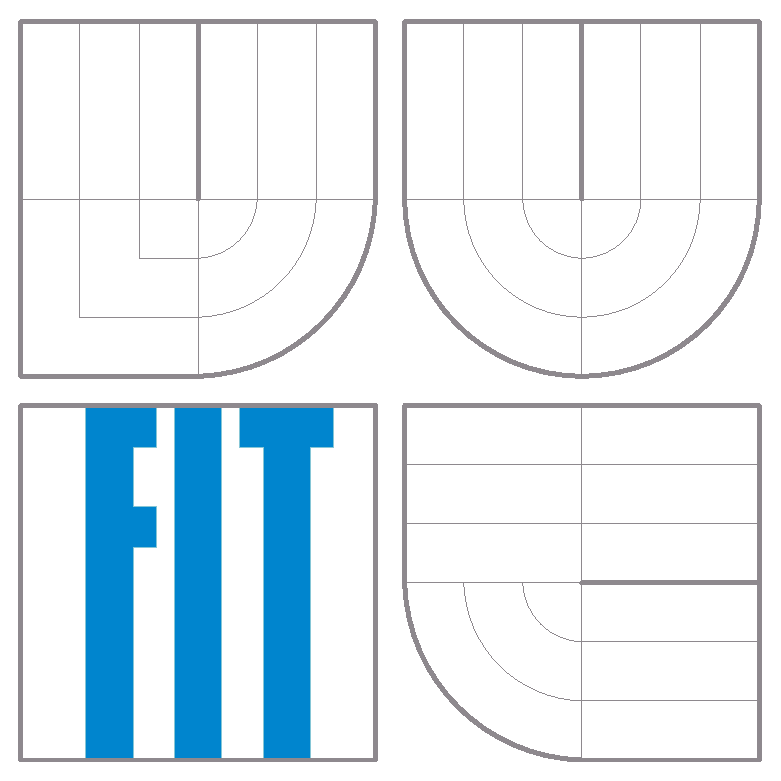
\includegraphics[height=5cm]{img/logo.eps}
\end{figure}

\vfill

\begin{center}
\begin{Large}
Dokumentace k projektu pro předměty IFJ a IAL\\
\end{Large}
\bigskip
\begin{Huge}
\projname\\
\end{Huge}
\begin{large}
Tým 113, varianta a/1/I\\
\end{large}
\textit{Vedoucí týmu: Antonín Marko}\\
\end{center}

\vfill

\begin{center}
\begin{Large}
\today
\end{Large}
\end{center}

\vfill

\begin{flushleft}
%\begin{large}
\begin{tabular}{l l l l l}
\textbf{Řešitelé}: 
&3BIT& Antonín Marko 20\% &\url{xmarko07@stud.fit.vutbr.cz} \\
&1BIT& Tomáš Pružina 20\% &\url{xpruzi01@stud.fit.vutbr.cz} \\
&3BIT& Martin Kubíček 20\% &\url{xkubic34@stud.fit.vutbr.cz} \\
&3BIT& Martin Juřík 20\% &\url{xjurik08@stud.fit.vutbr.cz} \\
&3BIT& Petr David 20\%s &\url{xdavid15@stud.fit.vutbr.cz} \\

%Autor: & \author, \url{\email}  \\
% & Fakulta Informačních Technologií \\
% & Vysoké Učení Technické v~Brně \\
\end{tabular}
\newline
\newline
\textbf{Rozšíření}: ARRAY, REPEAT, ELSEIF, BOOLOP, FOR
%\end{large}
\vfill
\begin{large}
Fakulta Informačních Technologií \\
Vysoké Učení Technické v~Brně \\
\end{large}
\end{flushleft}
\end{titlepage}

%%%%%%%%%%%%%%%%%%%%%%%%%%%%%%%%%%%%%%%%%%%%%%%%%%%%%%%%%%%%%%%%%%%%%%%%%%%%%%
% obsah
\pagestyle{plain}
\pagenumbering{roman}
\setcounter{page}{1}
\tableofcontents

%%%%%%%%%%%%%%%%%%%%%%%%%%%%%%%%%%%%%%%%%%%%%%%%%%%%%%%%%%%%%%%%%%%%%%%%%%%%%%
% textova zprava
\newpage
\pagestyle{plain}
\pagenumbering{arabic}
\setcounter{page}{1}

%%%%%%%%%%%%%%%%%%%%%%%%%%%%%%%%%%%%%%%%%%%%%%%%%%%%%%%%%%%%%%%%%%%%%%%%%%%%%%
\section{Úvod} \label{uvod}
%=============================================================================
Implementace překladače imperativního jazyka je netriviální úloha, proto je
vhodné ji rozdělit na podúlohy (\ref{moduly_interpretu}), které jsou vhodně
rozdělené mezi členy týmu, který je vedené a kontrolován týmovým vedoucím.

Tento dokument sa skládá z N částí, které popisují jednotlivé moduly
interpretu imperativního jazyka IFJ14, a to jsou lexikální analyzátor
(\ref{lexikalni_analyzator}), syntaktický analyzátor (\ref{syntakticky_analyzator})
využívající rekurzivní sestup (), který je pro potřeby syntaktické
analýzy výrazů rozšířený o Shunting-Yard (\ref{sya}) algoritmus.
Kontrola syntaxe a sémantiky probíhá z velké části při jednom průchodu, následné
kontroly sémantiky probíhají až za běhu.

%%%%%%%%%%%%%%%%%%%%%%%%%%%%%%%%%%%%%%%%%%%%%%%%%%%%%%%%%%%%%%%%%%%%%%%%%%%%%%
\section{Moduly interpretu jazyka} \label{moduly_interpretu}
%=============================================================================
\subsection{Lexikální analyzátor} \label{lexikalni_analyzator}

Syntaktický analyzátor potřebuje ke své činnosti lexikální analyzátor. Ten
předává na žádost syntaktického analyzátoru tzv. tokeny, které získává postupným
čtením vstupního souboru, který obsahuje zdrojový kód napsaný v jazyce IFJ14.
Samotný výsledný token je reprezentací lexému (identifikátor, klíčové slovo,
příkaz přiřazení atp.).

Pro úspěšné rozlišení typu lexému se v naší implementaci používá konečný
automat, jehož struktura je znázorněna na obrázku (\ref{lex_ka}).

Jestliže se konečný automat v době zpracovávání řetězce zdrojového souboru
document do chybového stavu \verb|lexerrref|, řetězec je nepřijatý a jedná se
o lexikální chybu. Samotná implementace lexikálního analyzátoru patří k
jednodušším částem projektu, avšak jeho návrh a testování zabralo nemálo času.

%<insert KA diagram here>
\begin{figure}\label{lex_ka}
	\centering
		%\includesvg{img/KA-scanner.svg}
	\caption{Konečný automat lexikálního analyzátoru}
\end{figure}

\subsection{Syntaktický analyzátor} \label{syntakticky_analyzator}
Jak již bylo zmíněno, syntaktický analyzátor žádá lexikální analyzátor o tokeny
a na základě sekvence po sobě jdoucích tokenů sestavuje abstraktní syntaktický
strom (dále jen AST). Tato sekvence musí odpovídat pravidlům syntaxe jazyka IFJ14,
v opačném případě se jedná o syntaktickou chybu.

Jazyk IFJ14 je staticky typovaný jazyk, tedy typové kontroly probíhají během 
překladu, v našem případě právě při průchodu syntaktickým analyzátorem. 

\subsubsection{Shunting-yard algoritmus} \label{sya}
\subsection{Interpret} \label{interpret}

Interpret je závěrečnou částí projektu. Rekurzivně zpracovává AST reprezentovaný
binárním stromem a postupně vykonává operace nad ním definované.

Kořenem tohoto AST je vždy typ převedené operace, přičemž obsahuje předem
definované nepovinné parametry (příkladem je podstrom volání funkce, který
obsahuje předávání proměnné). Tedy každý uzel AST představuje jednu atomickou
operaci, kterou je řízený samotný běh programu.

Interpret samozřejmě nepracuje jen se samotným syntaktickým stromem, ale
taktéž s tabulkou symbolů, která obsahuje data potřebná na to, aby interpret
mohl vykonávat nějakou užitočnou práci definovanou v těle programu.

Interpret tedy spravuje tabulky symbolů, dynamicky je za běhu
vykonávaného programu vytváří a (podla potřeby) ruší.

V neposlední řadě interpret vykonává sémantickou kontrolu u operacích, které
syntaktický analyzátor v době zpracování vstupního programu a generování
abstraktního syntaktického stromu neřešil.

Příkladem takovéto kontroly je používání (čtení) proměnné před její řádnou
definicí (přiřazením hodnoty) anebo dělení nulou v aritmetickém výrazu.

Takovéto běhové chyby jsou v interpretě řešené ukončením interpretace a navrácením
chybového kódu podle zadání imperativního jazyka IFJ14.

\subsubsection{Tabulka symbolů} \label{tabulka_symbolu}

Tabulka symbolů je implementována pomocí binárního vyhladávacího stromu,
přičemž se rozlišuje několik úrovní tabulky symbolů.

Každý program obsahuje globální tabulku symbolů (ve které jsou uložené ukazatele
na funkce) a lokální tabulku symbolů, která obsahuje běhové proměnné
vykonávaného programu.

Z implemetačního hlediska jsou lokální tabulky symbolů (stromy) ukládané na
zásobník, přičemž platí, že při volání funkce se vytvoří nová (lokální)
tabulka symbolů, do které se skopírují příslušné parametry volané funkce z
nižší vrstvy lokální tabulky (popř. z globální tabulky symbolů).

Taková lokální tabulka taktéž obsahuje návratovu hodnotu vykonávané funkce,
která umožňuje rekurzivní volání funkcí a samozřejmě umožňuje vykonávat tělo
funkce bez nutnosti jakkoliv zasahovat do abstraktního syntaktického stromu.


%%%%%%%%%%%%%%%%%%%%%%%%%%%%%%%%%%%%%%%%%%%%%%%%%%%%%%%%%%%%%%%%%%%%%%%%%%%%%%
\section{Postup při implementaci řešení} \label{postup_pri_implementaci_reseni}
%=============================================================================

%%%%%%%%%%%%%%%%%%%%%%%%%%%%%%%%%%%%%%%%%%%%%%%%%%%%%%%%%%%%%%%%%%%%%%%%%%%%%%
\section{Závěr} \label{zaver}
%%%%%%%%%%%%%%%%%%%%%%%%%%%%%%%%%%%%%%%%%%%%%%%%%%%%%%%%%%%%%%%%%%%%%%%%%%%%%

\appendix

\section{Metriky kódu} \label{metriky}

%%%%%%%%%%%%%%%%%%%%%%%%%%%%%%%%%%%%%%%%%%%%%%%%%%%%%%%%%%%%%%%%%%%%%%%%%%%%%%
% seznam citované literatury: každá položka je definována příkazem
% \bibitem{xyz}, kde xyz je identifikátor citace (v textu použij: \cite{xyz})
\begin{thebibliography}{1}

% jedna citace:
\bibitem{honzik}
HONZÍK J. M.: \emph{Studijní opora pro předmět Algoritmy}. Elektronický text. FIT VUT v Brně
\bibitem{meduna}
MEDUNA A., LUKÁŠ R., \emph{Podklady k přednáškám}. Elektronický text. FIT VUT v Brně


\end{thebibliography}
%%%%%%%%%%%%%%%%%%%%%%%%%%%%%%%%%%%%%%%%%%%%%%%%%%%%%%%%%%%%%%%%%%%%%%%%%%%%%%
\appendix

\end{document}
